
\section{Experimental results}\label{sec3}

This section offers a comprehensive overview of the dataset employed in the experiments, the evaluation metrics used to assess performance, and the experimental methodology adopted. The results of the experiments are presented through a combination of detailed plots and tables.

% =========================================== 
\subsection{Datasets}\label{sec:datasets}

Although numerous datasets are available for ABSA~\cite{ABSA_datasets}, the experiments in this notebook utilize the \texttt{SemEval2014Dataset} and \texttt{AmazonReviewsDataset}, which are described in more detail in the following. The sentiment distributions for these datasets are shown in Figure~\ref{fig:sentiment_distributions}.

\begin{figure}[h]
\centering
\begin{subfigure}{0.45\textwidth}
    \centering
    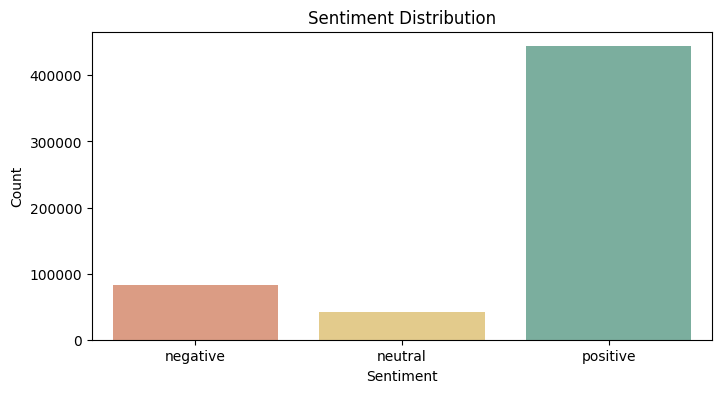
\includegraphics[width=\textwidth]{images/dist_amazon.png}
    \caption{Amazon Reviews Dataset}
    \label{fig:dist_amazon}
\end{subfigure}
\hfill
\begin{subfigure}{0.45\textwidth}
    \centering
    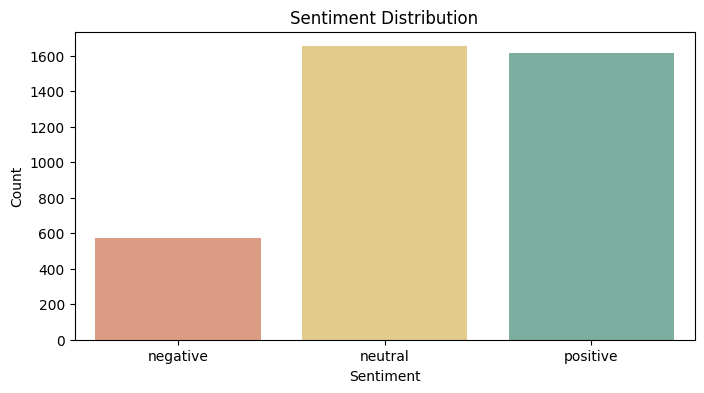
\includegraphics[width=\textwidth]{images/dist_semeval.png}
    \caption{SemEval2014 Dataset}
    \label{fig:dist_semeval}
\end{subfigure}
\caption{Distribution of negative, neutral, and positive sentiments in the datasets.}
\label{fig:sentiment_distributions}
\end{figure}

% ------------------------------------------- 
\subsubsection{\texttt{AmazonReviewsDataset}}

This dataset, available on Kaggle~\cite{amazon_dataset}, was used solely for experimenting with sentiment classification and is not specifically designed for aspect-based sentiment analysis. It contains approximately 500,000 reviews of fine foods from Amazon, each rated from 1 to 5. As the dataset only includes user-provided scores and our focus is on overall sentiment, the ratings were converted into sentiment categories: scores of 4 and 5 as \texttt{positive}, 3 as \texttt{neutral}, and 1 and 2 as \texttt{negative}.

The intuition behind selecting this dataset was that, as the \texttt{BornClassifier} is a statistical model, training on a larger corpus would likely improve its performance. The dataset was expected to expose the model to a broader vocabulary, with the \texttt{SemEval2014Dataset} serving as the test set, a topic which will be addressed subsequently.

% ------------------------------------------- 
\subsubsection{\texttt{SemEval2014Dataset}}

This dataset is a benchmark for aspect-based sentiment analysis tasks, and is accessible on HuggingFace~\cite{semeval2014_dataset}. While this repository provides two dataset categories, ``restaurants'' and ``laptops'' (both following the same format), our experiments were conducted solely on the ``restaurants'' dataset. This dataset contains a total of 7,886 rows, with each entry consisting of a given text, a list of aspect terms, and the corresponding sentiment associated with each of those aspects.

\texttt{SemEval2014Dataset} is primarily designed for aspect-based sentiment analysis. However, since it lacks overall sentiment labels for each document—necessary for the initial phase of the project involving sentiment classification with the \texttt{BornClassifier}—these labels were inferred based on the sentiments assigned to the aspects within each document. The labeling approach is as follows:

\begin{itemize}
    \item \texttt{positive}, if the number of positive aspects exceeds the number of negative aspects.
    \item \texttt{negative}, if the number of negative aspects exceeds the number of positive aspects.
    \item \texttt{neutral}, otherwise.
\end{itemize}

% =========================================== 
\subsection{Sentiment Analysis Evaluation}\label{sec:results_sentiment_analysis}

Table~\ref{tab:sentiment_analysis} compares the classification reports for all these experiments together. As our hypothesis regarding the effectiveness of training on \texttt{AmazonReviewsDataset} was rejected, we will proceed with the \texttt{BornClassifier} model which was trained on the training set of \texttt{SemEval2014Dataset}.

\begin{table}[h]
\caption{Comparison of Classification Reports Across Experiments}\label{tab:sentiment_analysis}
\begin{tabular*}{\textwidth}{@{\extracolsep{\fill}}lcccc}
\toprule
Class & Precision & Recall & F1-Score & Support \\
\midrule
Negative & 0.61 / \textcolor{purple}{0.51} / \textcolor{blue}{0.32} & 
0.71 / \textcolor{purple}{0.58} / \textcolor{blue}{0.51} & 
0.65 / \textcolor{purple}{0.55} / \textcolor{blue}{0.39} & 
16407 / \textcolor{purple}{125} / \textcolor{blue}{575} \\
Neutral & 0.29 / \textcolor{purple}{0.72} / \textcolor{blue}{0.47} & 
0.46 / \textcolor{purple}{0.57} / \textcolor{blue}{0.16} & 
0.36 / \textcolor{purple}{0.63} / \textcolor{blue}{0.24} & 
8528 / \textcolor{purple}{279} / \textcolor{blue}{1653} \\
Positive & 0.94 / \textcolor{purple}{0.74} / \textcolor{blue}{0.55} & 
0.86 / \textcolor{purple}{0.82} / \textcolor{blue}{0.80} & 
0.90 / \textcolor{purple}{0.78} / \textcolor{blue}{0.65} & 
88756 / \textcolor{purple}{396} / \textcolor{blue}{1613} \\
\midrule
Accuracy & & & 0.81 / \textcolor{purple}{0.70} / \textcolor{blue}{0.48} & 
113691 / \textcolor{purple}{800} / \textcolor{blue}{3841} \\
Macro Avg & 0.61 / \textcolor{purple}{0.66} / \textcolor{blue}{0.45} & 
0.67 / \textcolor{purple}{0.66} / \textcolor{blue}{0.49} & 
0.64 / \textcolor{purple}{0.65} / \textcolor{blue}{0.43} & 
113691 / \textcolor{purple}{800} / \textcolor{blue}{3841} \\
Weighted Avg & 0.84 / \textcolor{purple}{0.70} / \textcolor{blue}{0.48} & 
0.81 / \textcolor{purple}{0.70} / \textcolor{blue}{0.48} & 
0.82 / \textcolor{purple}{0.69} / \textcolor{blue}{0.44} & 
113691 / \textcolor{purple}{800} / \textcolor{blue}{3841} \\
\botrule
\end{tabular*}
\footnotetext{This table compares classification metrics across Experiment 1, \textcolor{purple}{Experiment 2}, and \textcolor{blue}{Experiment 3}.}
\end{table}


% ===========================================
\subsection{Aspect Detection Evaluation}

While evaluating predicted sentiments in both sentiment analysis and ABSA is relatively straightforward, the evaluation of aspect detection requires careful consideration. The key points to be taken into account are outlined below:

\begin{itemize}
    \item \textbf{Ground-truth aspect token length:} True aspects in the dataset are represented as noun phrases, some spanning up to six tokens, making even bigram or trigram tokenization insufficient for capturing all true aspects. To address this, a specialized function was employed to align candidate aspects with true aspects by shortening them to their minimal matching tokens, facilitating evaluation. For example, in the document \textit{``The pizza is the best if you like thin crusted pizza.''}, the true aspects \texttt{['pizza', 'thin crusted pizza']} and the predicted aspect \texttt{['pizza']} from our unigram-based detection algorithm were both reduced to \texttt{\{'pizza'\}}, resulting in an accurate interpretation of the document.

    \item \textbf{Evaluation metrics:} Each document contains tokens, some of which are \textit{true} aspects and others are not. According to the definitions provided below, aspect detection is evaluated by computing TP, FP, FN, and TN for each of documents, accumulating over all the given set of documents.
    \begin{itemize}
        \item \textbf{True Positive (TP):} Tokens in both \texttt{candidate\_set} and \texttt{true\_set}.
        
        \item \textbf{False Positive (FP):} Tokens in \texttt{candidate\_set} but not in \texttt{true\_set}.
        
        \item \textbf{False Negative (FN):} Tokens in \texttt{true\_set} but not in \texttt{candidate\_set}.
        
        \item \textbf{True Negative (TN):} Tokens except in \texttt{candidate\_set} and \texttt{true\_set}.
    \end{itemize}
\end{itemize}

The formulas for the evaluation metrics are defined below:

\begin{equation*}
\begin{aligned}
\text{Accuracy} & = \frac{TP + TN}{TP + TN + FP + FN}, \\
\text{Precision} & =
\begin{cases}
\frac{TP}{TP + FP}, & \text{if } TP + FP > 0, \\
0, & \text{otherwise},
\end{cases} \\
\text{Recall} & =
\begin{cases}
\frac{TP}{TP + FN}, & \text{if } TP + FN > 0, \\
0, & \text{otherwise},
\end{cases} \\
F_1 & =
\begin{cases}
\frac{2 \cdot \text{Precision} \cdot \text{Recall}}{\text{Precision} + \text{Recall}}, & \text{if } \text{Precision} + \text{Recall} > 0, \\
0, & \text{otherwise}.
\end{cases}
\end{aligned}
\end{equation*}

On the test set, with the same optimal \texttt{best\_aspect\_threshold} found in Section~\ref{sec:aspect_detection}, we achieved an accuracy of \texttt{0.918509}, precision \texttt{0.548289}, recall \texttt{0.800893}, and F1-score of \texttt{0.650943} in detecting the aspects.


% ===========================================
\subsection{Aspect-Based Sentiment Analysis Evaluation}

It is evident that our \texttt{AspectDetection} algorithm is not optimal, meaning it does not accurately identify all aspects. As a result, there may be detected aspects without corresponding ground-truth sentiments, or true aspects that our algorithm fails to detect.

To address this limitation, we evaluated sentiment prediction for aspects independently of the aspect detection process. In other words, we did not rely on the candidate aspects detected by our algorithm for aspect-based sentiment analysis. Instead, we assumed the availability of a perfect algorithm capable of identifying all true aspects correctly. Using this ground-truth set of aspects, we proceeded to evaluate sentiment predictions for the text portions where each aspect appeared, which were identified according to Section~\ref{sec:aspect_to_sent}. 

Table~\ref{tab:born_aspect_based} summarizes the performance in predicting the sentiment for each text portion, reporting the results over the whole dataset (train and test combined).

\begin{table}[h]
\caption{Performance of \texttt{BornClassifier} in Aspect-based Sentiment Analysis}\label{tab:born_aspect_based}%
\begin{tabular*}{\textwidth}{@{\extracolsep{\fill}}lcccc}
\toprule
Class & Precision & Recall & F1-Score & Support \\
\midrule
Negative & 0.68 & 0.80 & 0.73 & 1001 \\
Neutral & 0.55 & 0.31 & 0.40 & 828 \\
Positive & 0.85 & 0.91 & 0.88 & 2874 \\
\midrule
Accuracy & & & 0.78 & 4703 \\
Macro Avg & 0.70 & 0.67 & 0.67 & 4703 \\
Weighted Avg & 0.76 & 0.78 & 0.76 & 4703 \\
\botrule
\end{tabular*}
\end{table}


% ===========================================
\subsection{Experiments with Large Language Models (LLMs)}\label{section:llms}

To provide a more thorough analysis in this study, our final attempt is to evaluate the sentiment prediction leveraging LLMs. This includes assessing both overall sentiment prediction for entire documents and aspect-based sentiment analysis within specific text portions. Finally, we compare the obtained results with those of \texttt{BornClassifer}.

The large language models used for comparison are listed as below:
\begin{itemize}
    \item \textbf{NLTK's \texttt{SentimentIntensityAnalyzer} model:} This model assigns a sentiment intensity score to sentences, returning a float for sentiment strength based on the input text~\cite{llm_nltk}.

    \item \textbf{HuggingFace's \texttt{RoBERTa} model:} This RoBERTa-base model has been trained on nearly 58M tweets and fine-tuned for sentiment analysis with the TweetEval benchmark. It returns a sentiment score for each of the negative, neutral, and positive cases~\cite{llm_roberta}.
\end{itemize}

Tables~\ref{tab:llm_sentiment} and \ref{tab:llm_absa} compare the performance of these LLMs in both sentiment analysis and aspect-based sentiment analysis, respectively.

\begin{table}[h]
    \caption{NLTK vs. \textcolor{blue}{RoBERTa} in Sentiment Analysis}\label{tab:llm_sentiment}
    \begin{tabular*}{\textwidth}{@{\extracolsep{\fill}}lcccc}
    \toprule
    Class & Precision & Recall & F1-Score & Support \\
    \midrule
    Negative & 0.45 / \textcolor{blue}{0.51} & 0.41 / \textcolor{blue}{0.67} & 0.43 / \textcolor{blue}{0.58} & 575 \\
    Neutral & 0.59 / \textcolor{blue}{0.64} & 0.36 / \textcolor{blue}{0.37} & 0.45 / \textcolor{blue}{0.47} & 1653 \\
    Positive & 0.57 / \textcolor{blue}{0.65} & 0.82 / \textcolor{blue}{0.85} & 0.67 / \textcolor{blue}{0.74} & 1613 \\
    \midrule
    Accuracy & & & 0.56 / \textcolor{blue}{0.62} & 3841 \\
    Macro Avg & 0.54 / \textcolor{blue}{0.60} & 0.53 / \textcolor{blue}{0.63} & 0.52 / \textcolor{blue}{0.59} & 3841 \\
    Weighted Avg & 0.56 / \textcolor{blue}{0.62} & 0.56 / \textcolor{blue}{0.62} & 0.54 / \textcolor{blue}{0.60} & 3841 \\
    \botrule
    \end{tabular*}
\end{table}

\begin{table}[h]
    \caption{NLTK vs. \textcolor{blue}{RoBERTa} in Aspect-based Sentiment Analysis}\label{tab:llm_absa}
    \begin{tabular*}{\textwidth}{@{\extracolsep{\fill}}lcccc}
    \toprule
    Class & Precision & Recall & F1-Score & Support \\
    \midrule
    Negative & 0.65 / \textcolor{blue}{0.72} & 0.39 / \textcolor{blue}{0.63} & 0.49 / \textcolor{blue}{0.67} & 1001 \\
    Neutral & 0.33 / \textcolor{blue}{0.38} & 0.45 / \textcolor{blue}{0.52} & 0.38 / \textcolor{blue}{0.44} & 828 \\
    Positive & 0.78 / \textcolor{blue}{0.87} & 0.80 / \textcolor{blue}{0.82} & 0.79 / \textcolor{blue}{0.84} & 2874 \\
    \midrule
    Accuracy & & & 0.65 / \textcolor{blue}{0.73} & 4703 \\
    Macro Avg & 0.58 / \textcolor{blue}{0.66} & 0.55 / \textcolor{blue}{0.66} & 0.55 / \textcolor{blue}{0.65} & 4703 \\
    Weighted Avg & 0.67 / \textcolor{blue}{0.75} & 0.65 / \textcolor{blue}{0.73} & 0.65 / \textcolor{blue}{0.74} & 4703 \\
    \botrule
    \end{tabular*}
\end{table}

In both scenarios of sentiment analysis and aspect-based sentiment analysis, it is clear that the \texttt{BornClassifier} has demonstrated superior performance compared to both the NLTK and RoBERTa models.